\section{[Completed] Better Pivots}

To make a metal bar turn with an axle, a lock bar was needed so that the rotational speed was transferred. However, as it turns out, the 84-tooth gear has holes for screws that allow you to directly screw the gear onto the metal bar so that it replaces the role of the lock bar. With this discovery, two 84-tooth gears are now able to fit in the arm support.

\begin{figure}[h]
    \centering
    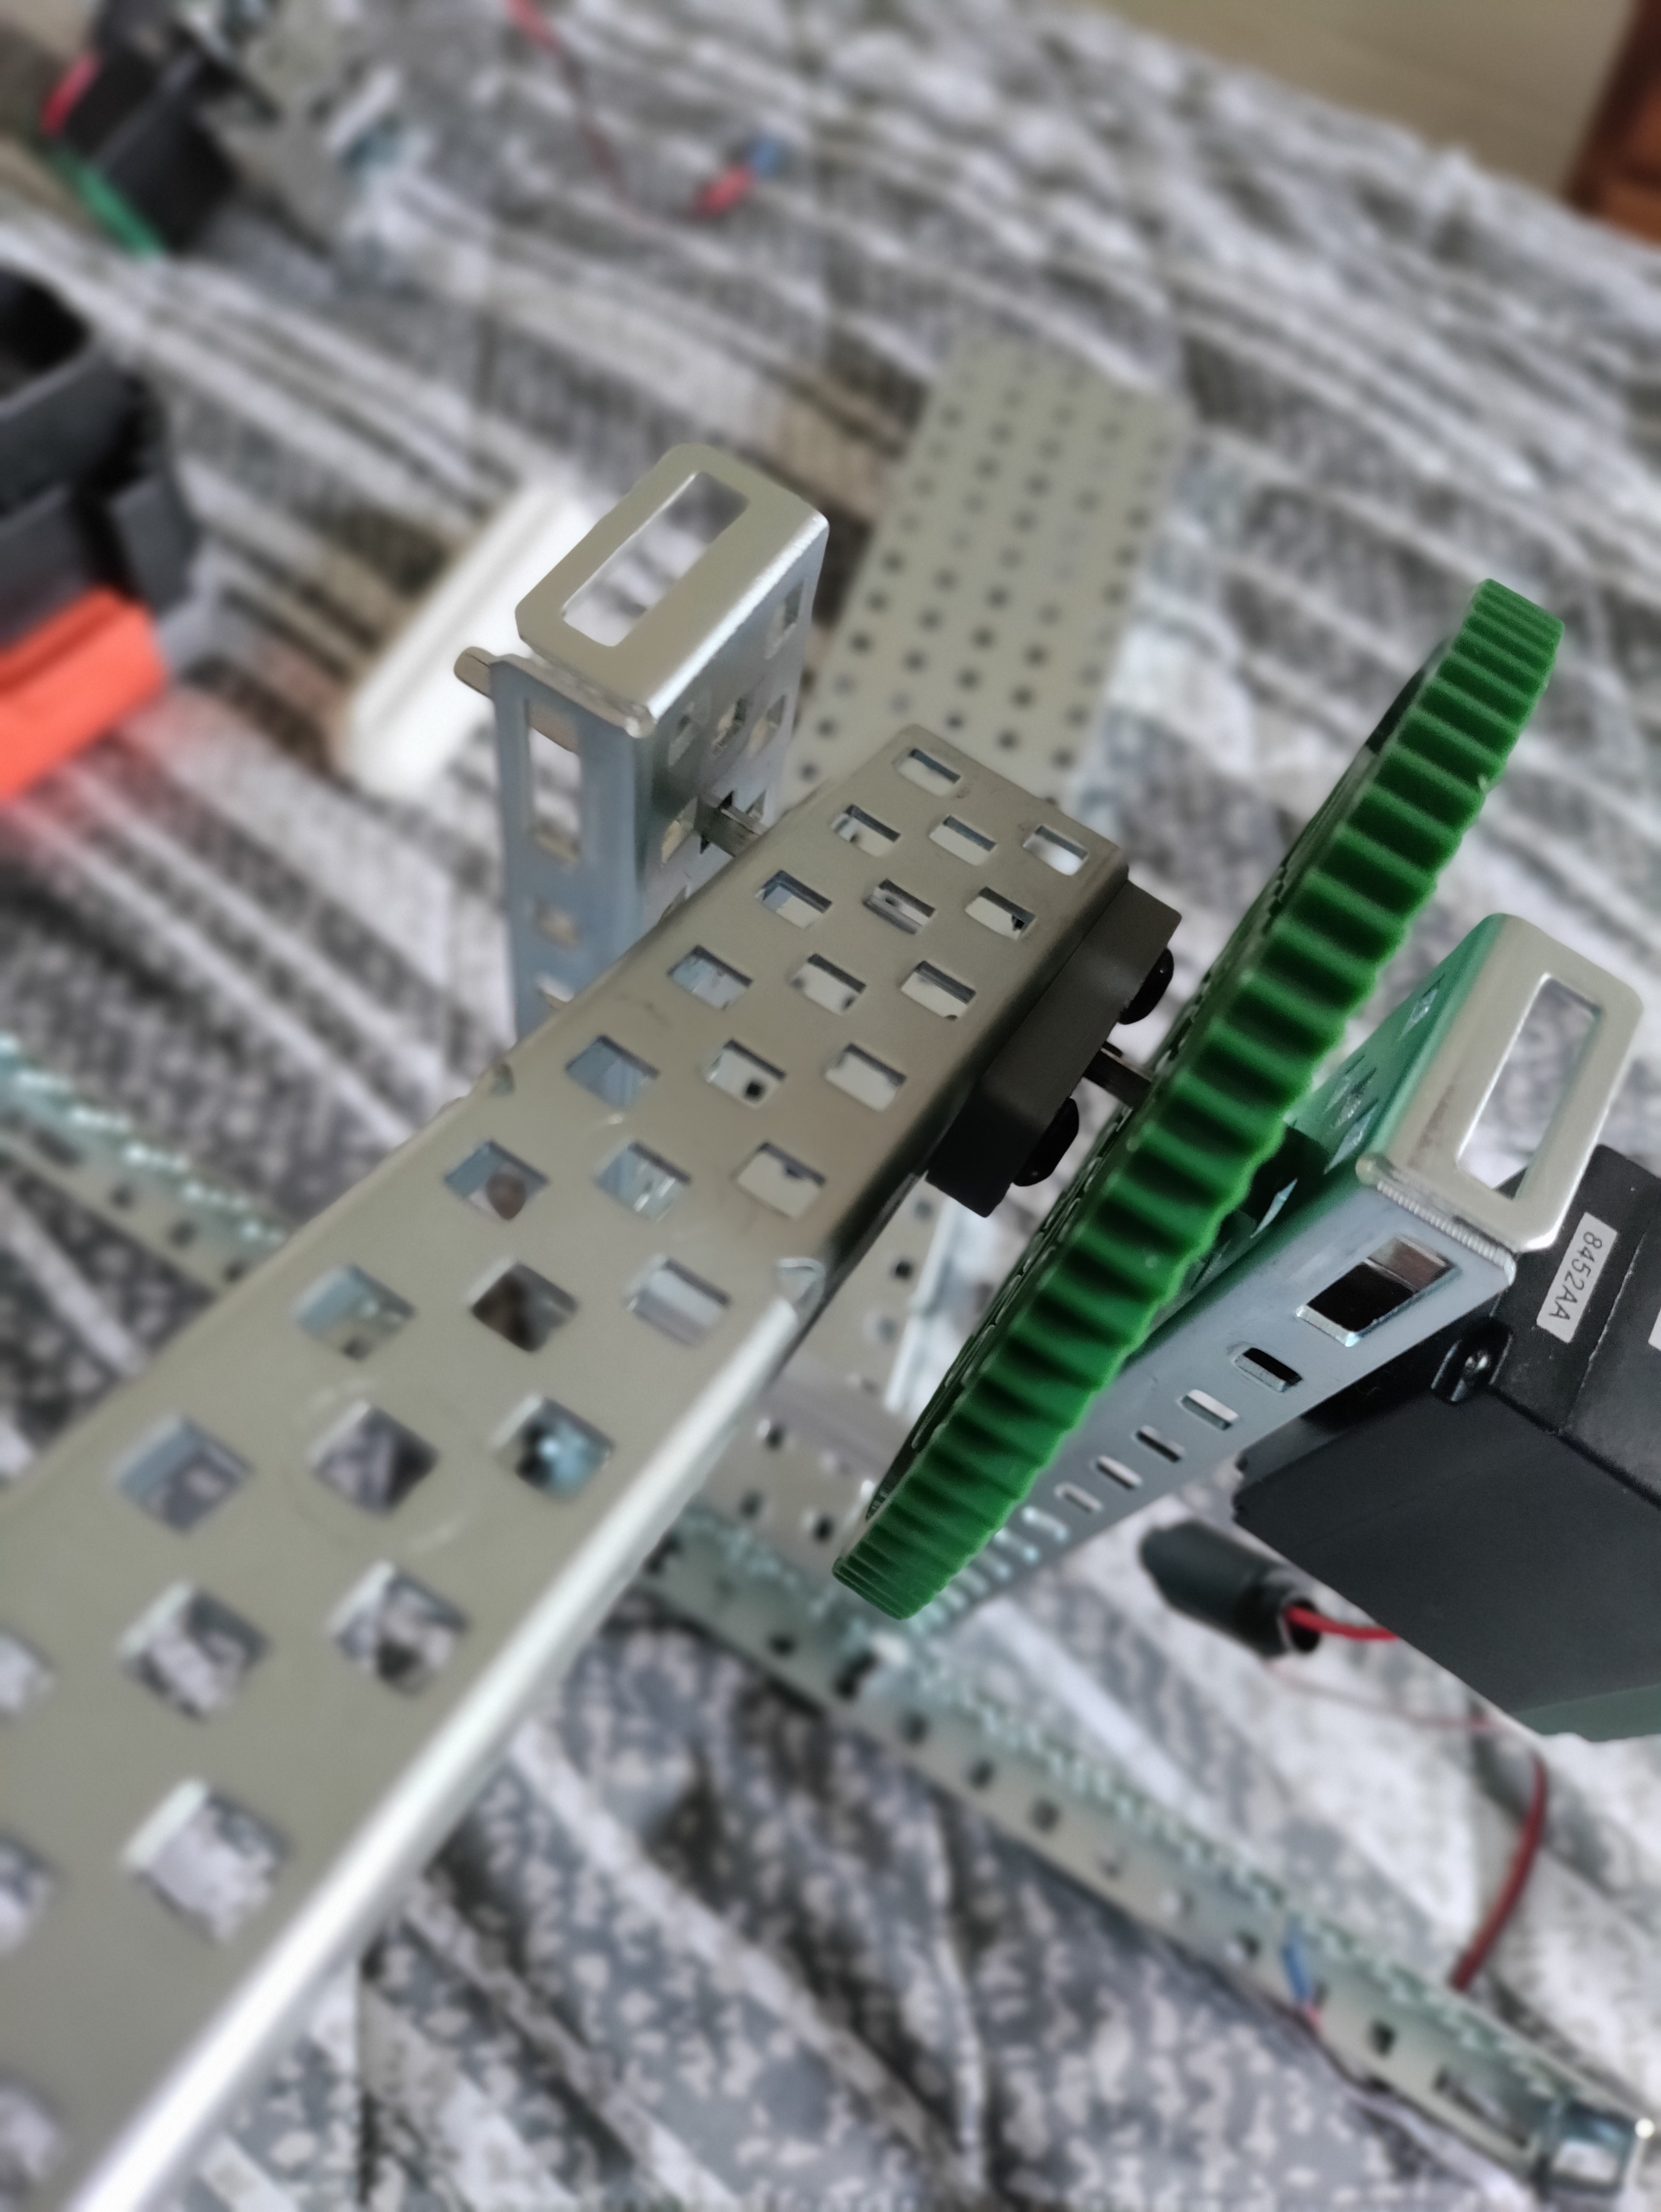
\includegraphics[width=\textwidth,height=5cm,keepaspectratio=true]{Pivot/lockandgear}
    \caption{
        What we used previously; A lock bar attached to metal with a gear in parallel. With this design, you could only fit 1 84-tooth gear, 2 if you very carefully screwed the lock bar on the inside of the c-channel.
    }
\end{figure}

\begin{figure}[h]
    \centering
    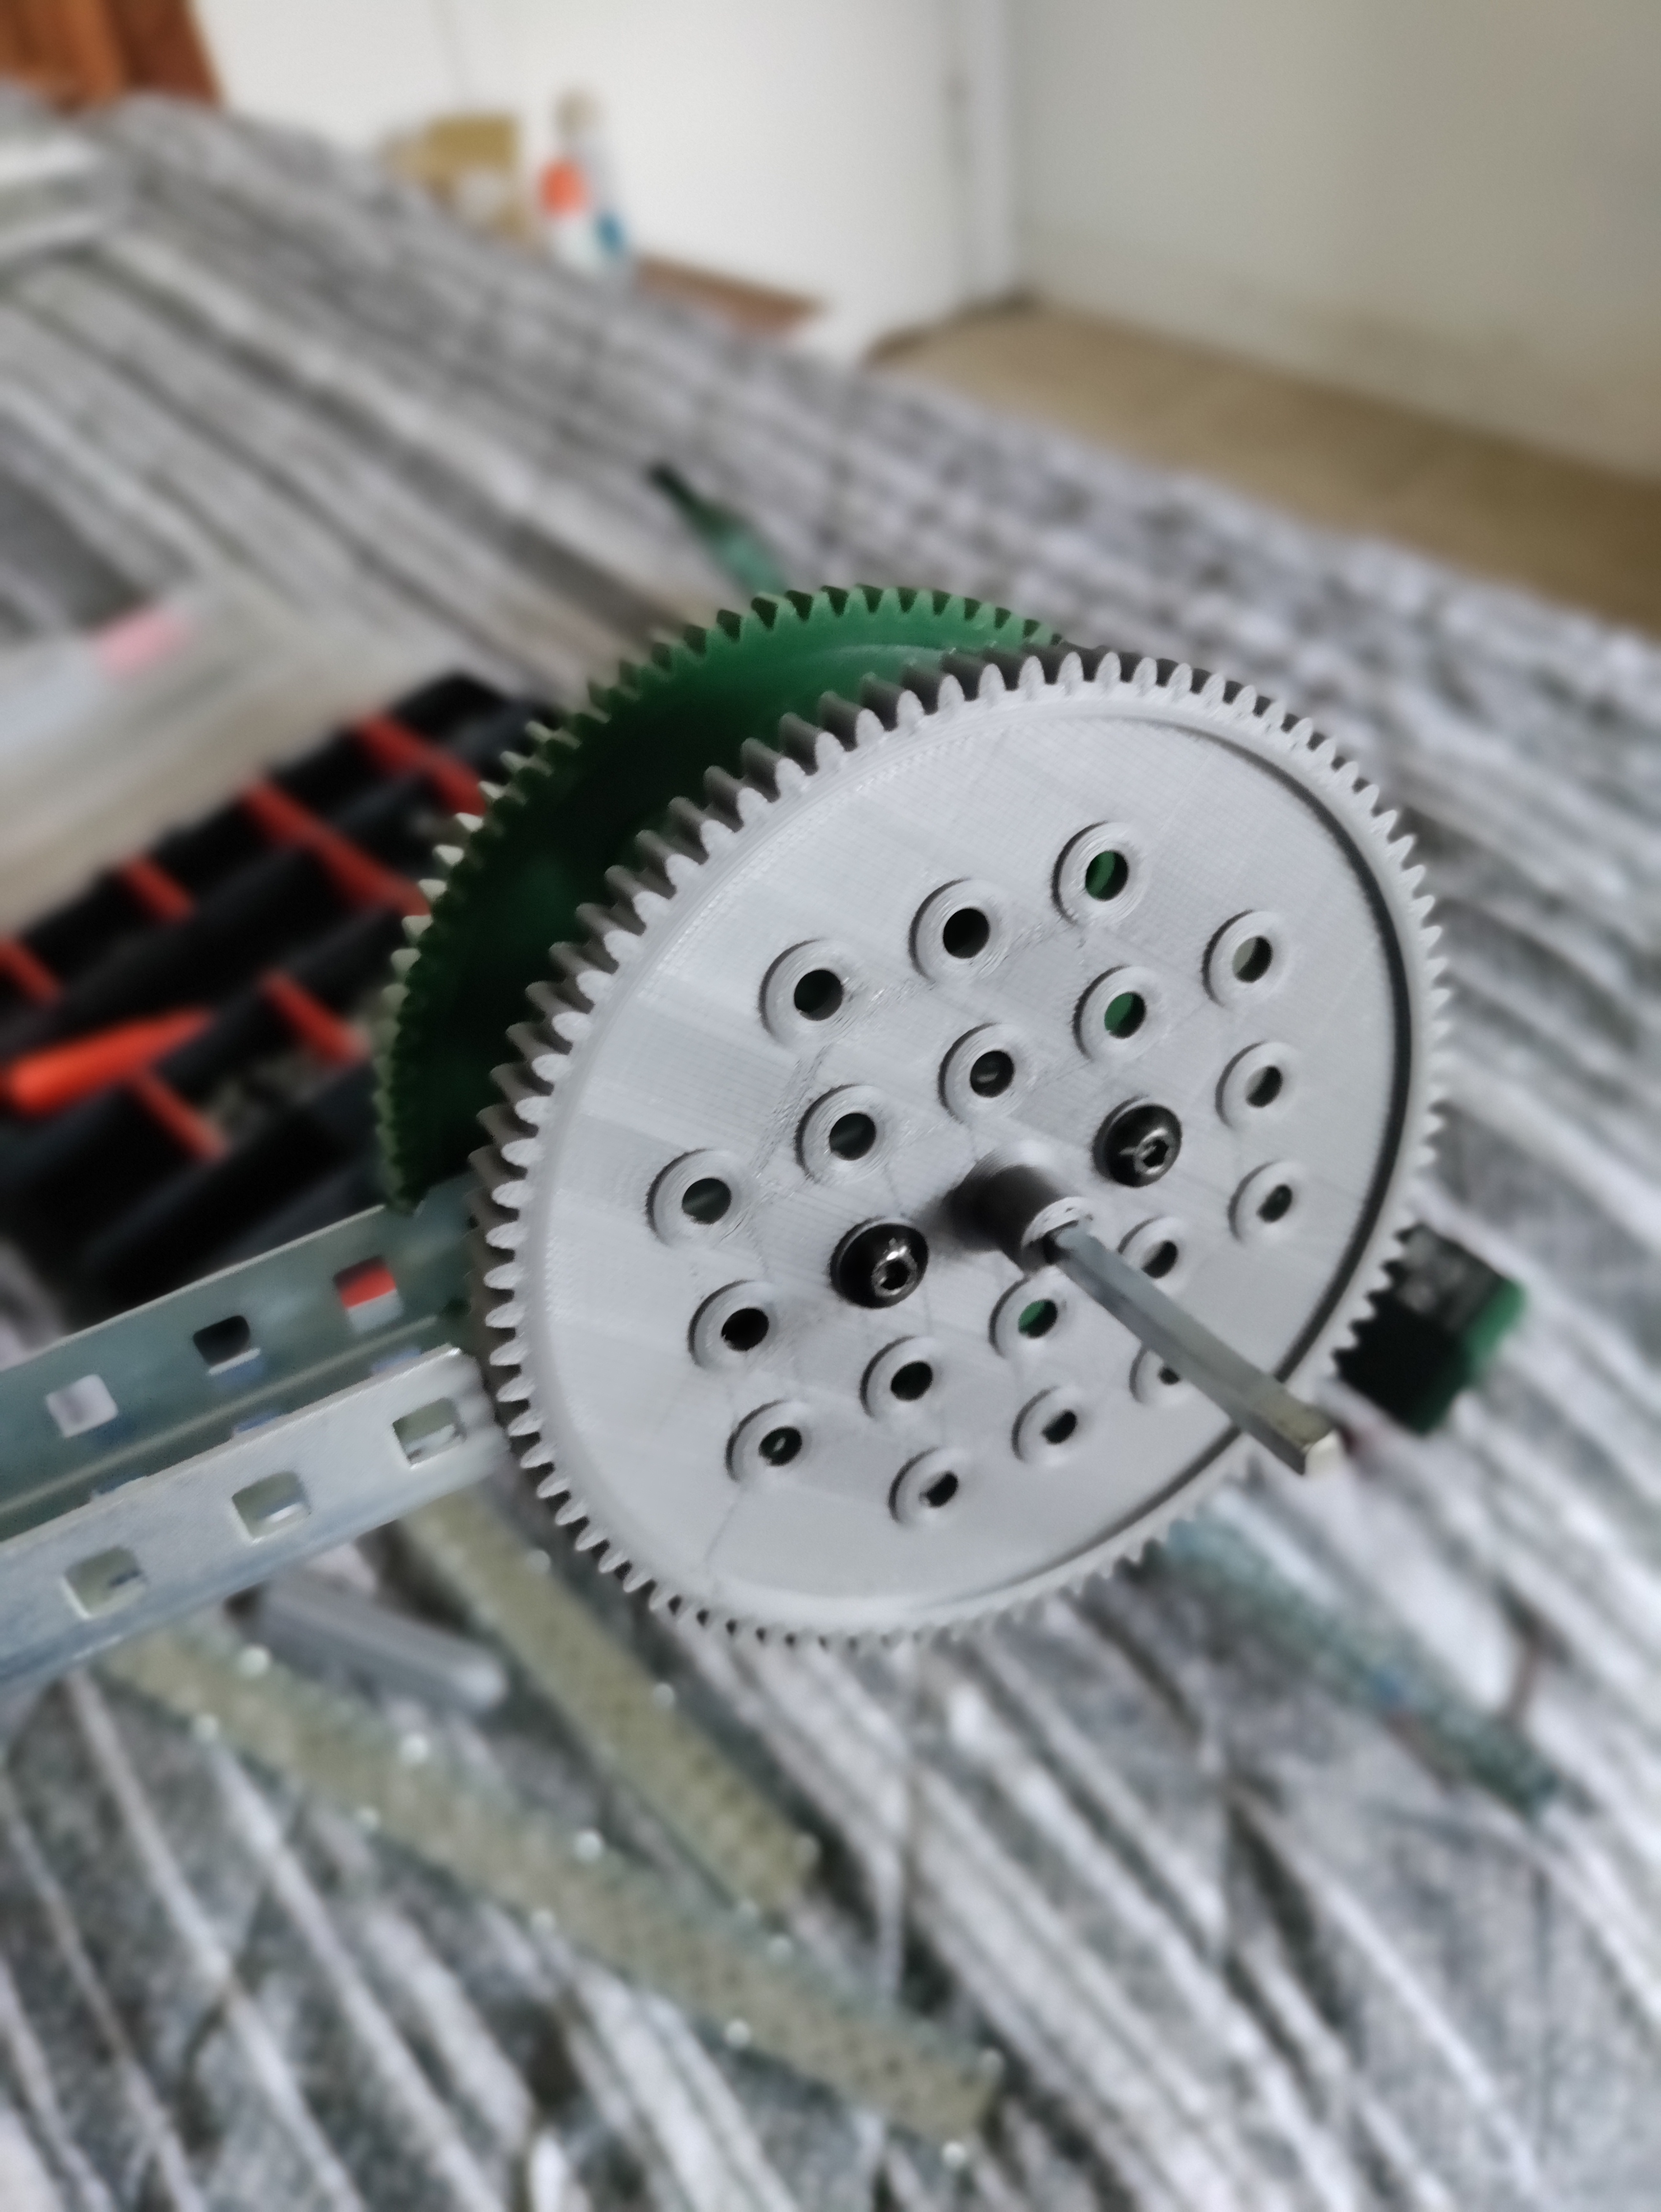
\includegraphics[width=\textwidth,height=5cm,keepaspectratio=true]{Pivot/gearandgear1}
    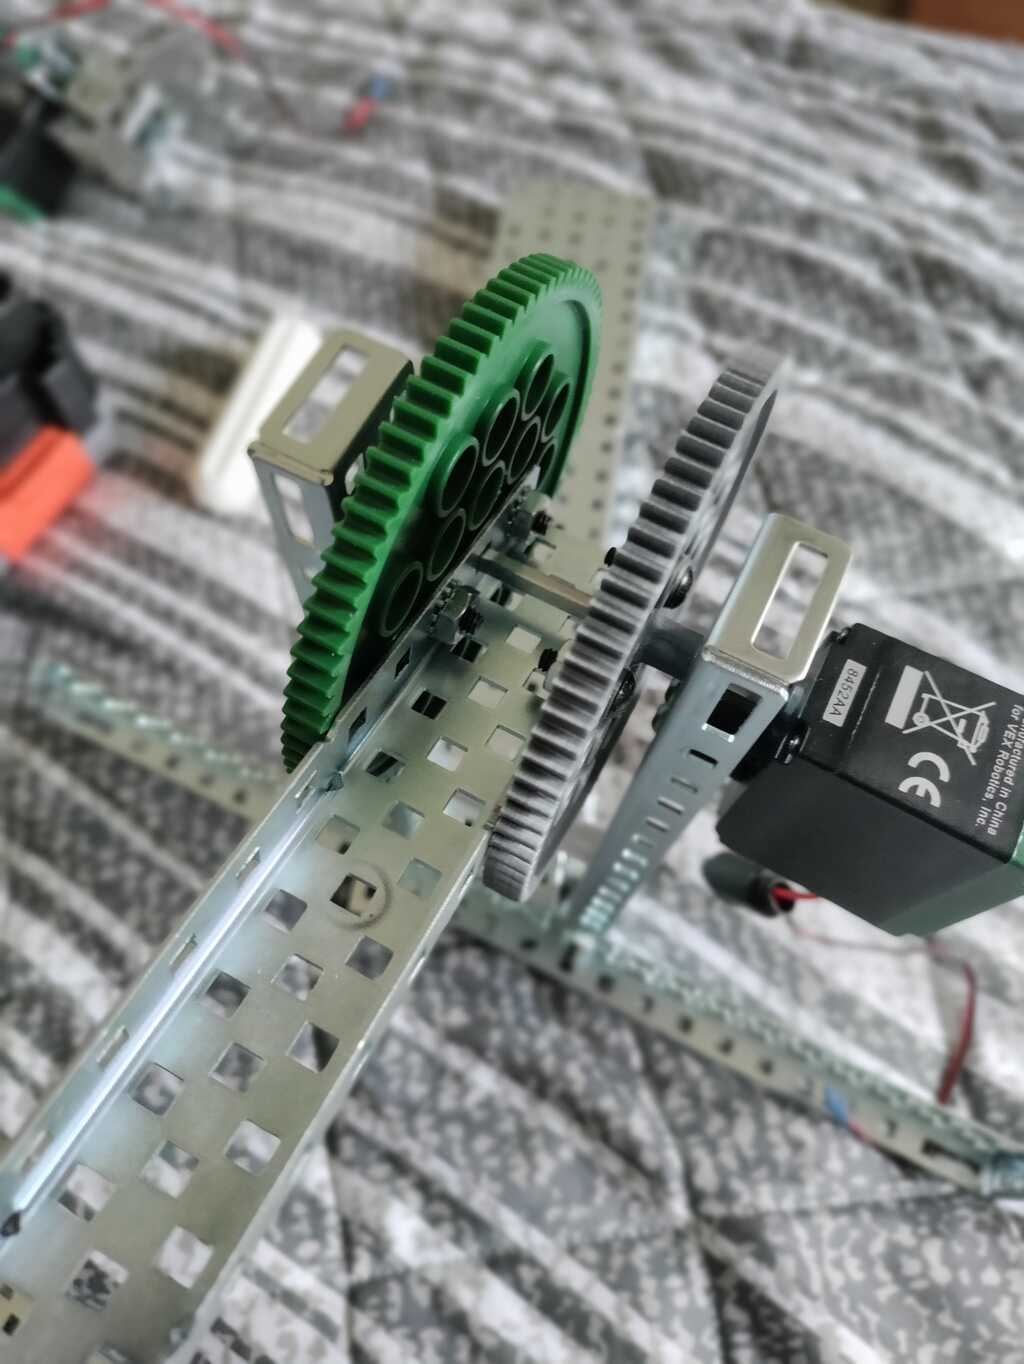
\includegraphics[width=\textwidth,height=5cm,keepaspectratio=true]{Pivot/gearandgear2}
    \caption{
        (Left) Two gears being screwed to a c-channel so that it acts like a lock bar. (Right) The two gears are able to fit the support for the arm with no problem.
    }
\end{figure}
